Da die Anregung über die Ionisation dominiert, ist der Energieverlust, der zur Ionisation nötig ist,
größer als die Ionisationsenergie des Atoms. Die mittlere Anzahl der Elektron-Ion-Paare ist gegeben
durch

\[\frac{\text{Energieverlust des Teilchens}}{\text{mittlere Energie für die Erzeugung eines
$e^-$-Ion-Paares}} \]

Typische Werte für die benötigte Energie sind etwa $30\,$eV. So erzeugt ein $3\,$keV-Teilchen etwa
$\frac{3000\,\text{eV}}{30\,\text{eV}}=100$ $e^-$-Ion-Paare.

\begin{figure}[H]
	\centering
	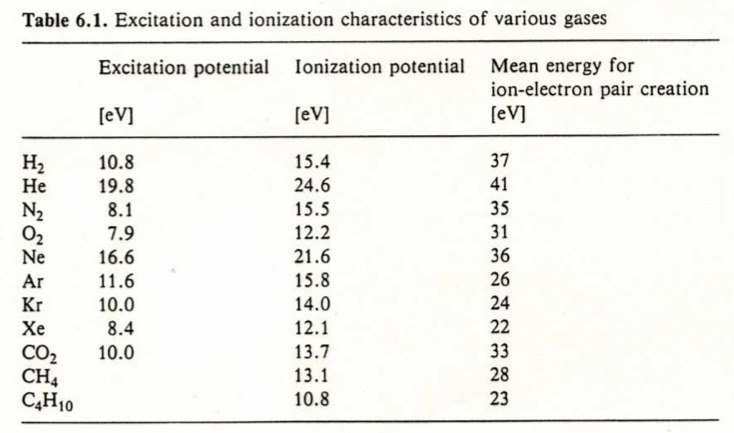
\includegraphics[width=0.5\textwidth]{Fig-03-01.jpg}
\end{figure}

Das Ziel ist die Bestimmung des Energieverlustes von Teilchen. Die Idee ist dabei, die Anzahl der
erzeugten $e^-$-Ion-Paare zu bestimmen - wobei gilt: je größer die Anzahl, desto genauer die
Messung.

\[\text{Teilchenenergie}\approx \#(\text{$e^-$-Ion-Paare})\cdot (\text{mittlere Energie für ein
$e^-$-Ion-Paar})\]

Für eine Anzahl $N_{\text{Mess}}\ge 20$ ergibt sich bei wiederholter Messung der erzeugten primären
Gesamtionisation (???) eine Gaußkurve

\begin{figure}[H]
	\centering
	
\includegraphics[width=0.5\textwidth]{dummy.jpg}
\end{figure}

Die relative Auflösung entspricht in diesem Fall

\[\frac{\sigma_{a}}{\langle a \rangle} =
\frac{\sqrt{N_{\text{Mess}}}}{N_{\text{Mess}}}=\frac{1}{\sqrt{N_{\text{Mess}}}}
\]

als bestmöglichste Auflösung für einen rein statistischen Prozess. Tatsächlich ergeben sich kleine
Werte, und zwar um den sogenannten Fano-Faktor $F$:

\[ F:=\frac{\text{beobachtete Auflösung}}{\text{erwartete Auflösung (aus Poisson-Statistik)}} \]

Beispiele:

\ldots

Die Ionisationsprozesse sind nicht statistisch unabhängig!

